%%%%%%%%%%%%%%%%%%%%%%%%%%%%%%%%%%%%%%%%%
% ENSAE Assignment Title Page 
% LaTeX Template
% Version 1.0 (27/12/12)
%
% This template has been downloaded from:
% http://www.LaTeXTemplates.com
%
% Original author:
% WikiBooks (http://en.wikibooks.org/wiki/LaTeX/Title_Creation)
% Modified by Julien Perrin to fit ENSAE
% License:
% 
%----------------------------------------------------------------------------------------
%	PACKAGES AND OTHER DOCUMENT CONFIGURATIONS
%----------------------------------------------------------------------------------------


\documentclass[12pt]{article}
\usepackage[letter, left=1in, right=1in, top=1in, bottom=1.5in]{geometry}
\usepackage[spanish]{babel}
\usepackage[utf8x]{inputenc}
\usepackage{amsmath}
\usepackage[natbibapa]{apacite}
\usepackage{graphicx}
\usepackage{float}
\usepackage{dsfont}
\usepackage{tocstyle}
\usepackage{multicol}
\usepackage{setspace}
\usepackage{amsfonts}
\usepackage{appendix}
\usepackage[T1]{fontenc}
\usepackage[colorinlistoftodos]{todonotes}
\usepackage{minted}
\usepackage{listings}
\usepackage[usenames,dvipsnames]{xcolor}
\usepackage{tcolorbox}
\usepackage{tabularx}
\usepackage{array}
\usepackage{colortbl}
\tcbuselibrary{skins}

\newcolumntype{Y}{>{\raggedleft\arraybackslash}X}
\newcolumntype{f}{>{\hsize=.36\hsize}Y}
\newcolumntype{s}{>{\hsize=.36\hsize}X}
\newcolumntype{t}{>{\hsize=1\hsize}X}

\tcbset{tab1/.style={fonttitle=\bfseries\large,fontupper=\normalsize\sffamily,
colback=yellow!10!white,colframe=red!75!black,colbacktitle=Salmon!40!white,
coltitle=black,center title,freelance,frame code={
\foreach \n in {north east,north west,south east,south west}
{\path [fill=red!75!black] (interior.\n) circle (3mm); };},}}

\tcbset{tab2/.style={enhanced,fonttitle=\bfseries,fontupper=\normalsize\sffamily,
colback=yellow!10!white,colframe=red!50!black,colbacktitle=Salmon!40!white,
coltitle=black,center title}}

\newcommand{\source}[1]{\caption*{Fuente: {\textit{#1}}} }

\newcommand{\deriv}{\mathrm{d}}
\lstset{
    language=Python,
    basicstyle=\SSEiptsize\ttfamily,
    commentstyle=\ttfamily\color{red},
    numbers=left,
    numberstyle=\ttfamily\color{blue}\footnotesize,
    stepnumber=1,
    numbersep=5pt,
    backgroundcolor=\color{white},
    showspaces=false,
    showstringspaces=false,
    showtabs=false,
    frame=single,
    tabsize=2,
    captionpos=b,
    breaklines=true,
    breakatwhitespace=false,
    title=\lstname,
    escapeinside={},
    keywordstyle={},
    morekeywords={}
    }

    
\usepackage{caption}
\usepackage{subcaption}   
\usepackage{parskip}
    
    
\usepackage{color}   %May be necessary if you want to color links
\usepackage{hyperref}
\hypersetup{
    colorlinks=true, %set true if you want colored links
    linktoc=all,     %set to all if you want both sections and subsections linked
    linkcolor=blue,  %choose some color if you want links to stand out
    citecolor=gray,  %choose some color if you want citations to stand out
}




\usetocstyle{standard}





\usepackage{xcolor}
\definecolor{tssteelblue}{RGB}{70,130,180}





\usepackage{sectsty}
\sectionfont{\sf\color{tssteelblue}\sectionrule{0ex}{0pt}{-1ex}{1pt}}






\usepackage{fancyhdr}
\fancypagestyle{firstpage}
{
    \fancyhead[L]{
\includegraphics[width=6cm]{logotipo-FAE-1.png}}    
    \fancyhead[R]{}
    \fancyfoot{}
}

\fancypagestyle{toc-style}
{
    \fancyhead[R]{
\includegraphics[width=3cm]{logotipo-FAE-1.png}}
    \pagenumbering{alph}
    \fancyfoot[c]{Índice - Página (\thepage)}
}

\fancypagestyle{Content}
{
    \fancyhead[R]{
\includegraphics[width=3cm]{logotipo-FAE-1.png}}
    \pagenumbering{arabic}
    \fancyfoot[c]{Página (\thepage)}
}

\fancypagestyle{Ref}
{
    \fancyhead[R]{
\includegraphics[width=3cm]{logotipo-FAE-1.png}}
    \pagenumbering{Roman}
    \fancyfoot[c]{Página (\thepage)}
}







\title{Tarea No.1}

\begin{document}
\renewcommand{\listfigurename}{Índice de Figuras}
\renewcommand{\listtablename}{Índice de Tablas}
\renewcommand{\tablename}{Tabla}

\begin{titlepage}

\newcommand{\HRule}{\rule{\linewidth}{0.2mm}} % Defines a new command for the horizontal lines, change thickness here

\center % Center everything on the page
 
%----------------------------------------------------------------------------------------
%	HEADING SECTIONS
%----------------------------------------------------------------------------------------

\thispagestyle{firstpage}

\textsc{\LARGE }\\[3cm]
\textsc{\Large Módulo 3}\\[0.5cm] % Major heading such as course name
\textsc{\large Estadística para Data Science}\\[1.5cm] % Minor heading such as course title

%----------------------------------------------------------------------------------------
%	TITLE SECTION
%----------------------------------------------------------------------------------------

\HRule \\[0.7cm]
{ \huge \bfseries Evidenciando el calentamiento global}\\[0.2cm]
{\large Análisis estadístico del cambio de temperatura}\\[0.4cm]% Title of your document
\HRule \\[5.5cm]
 
%----------------------------------------------------------------------------------------
%	AUTHOR SECTION
%----------------------------------------------------------------------------------------
\flushleft
\begin{minipage}{0.6\textwidth}
\begin{flushleft} \large
\textbf{}\\
\hskip 1cm Patricio \textsc{Mallea} (18.486.857-1)\\
% Your name
\end{flushleft}

\end{minipage}\\[4cm]

% If you don't want a supervisor, uncomment the two lines below and remove the section above
%\Large \emph{Author:}\\
%John \textsc{Smith}\\[3cm] % Your name

%----------------------------------------------------------------------------------------
%	DATE SECTION
%----------------------------------------------------------------------------------------
\center 
{\large \today}\\[2cm] % Date, change the \today to a set date if you want to be precise

\vfill % Fill the rest of the page with whitespace
\end{titlepage}

%----------------------------------------------------------------------------------------
%	TABLE OF CONTENTS
%------------------------------

\newpage
\thispagestyle{toc-style}
\tableofcontents
\listoffigures
\listoftables


%----------------------------------------------------------------------------------------
%	PROBLEM 1
%------------------------------
\newpage
\clearpage
\pagenumbering{arabic}
\pagestyle{Content}
\section{Introducción}
Cuando nos preguntamos acerca de una de principales problemática del siglo XXI las opiniones confluyen en el abrupto cambio climático producto del accionar desmedido de los seres humanos. El propósito de este analísis es revisar de manera cuantitativa como las temperaturas se han elevado abruptamente con el pasar del tiempo mediante una base de datos obtenida en el sitio web de la Organización de las Naciones Unidas para la Alimentación y la Agricultura o \cite{fao_site} que da cuenta de los cambios de temperatura mensual con respecto al año anterior desde el año 1961 hasta el año 2020 en los distintos países del mundo .\\ \\
Mediante una mirada generalísima, el cambio climático puede ser definido según la CEPAL como “La variación global del clima de la Tierra debido a causas naturales, pero principalmente a la acción humana, que se traduce en quema de combustibles fósiles, pérdida de bosques y otras actividades producidas en el ámbito industrial, agrícola y transporte, entre otros, como consecuencia de una retención del calor del Sol en la atmósfera.” A su vez, el IPCC lo define como “una modificación en el estado del clima que mediante el uso de pruebas estadísticas cambios en la media y/o la variabilidad de sus propiedades y que persiste durante un periodo prolongado, típicamente décadas o más.”. \\ \\
Es radicalmente importante conocer de este hecho, dado que cuenta con el carácter de multidimensional, es patente como podemos caer en cuenta que la degradación del medioambiente trae consigo numerosas consecuencias como son la pobreza, la generación de zonas de sacrificio, emperoamiento de la calidad de vida de las personas, afectación en la salud, la afectación de actividades económicas extractivas, etc. Además posee multiescalaridad, dado que al ser tan complejo debemos adoptar un enfoque interdisciplinario que nos permita abordarlo en su totalidad, es así como disciplinas tan disímiles como son las ciencias naturales con las ciencias sociales deben trabajar al unísono con miras a un objetivo común.\\ \\
La ONU por medio del informe más completo hasta la fecha anunció que el cambio climático es ya irreversible, significando esto una alerta roja para la humanidad. El Panel Intergubernamental de Expertos sobre el Cambio Climático* (IPCC, por sus siglas en inglés) evaluó cómo el calentamiento global cambiará el mundo en las próximas décadas tras examinar más de 14.000 artículos científicos.  También creen que "no es posible descartar" una subida del nivel del mar que se acerque a los 2 metros a finales de este siglo.\\ \\
Según la WWF, las principales causas del cambio climático en el mundo son: las crecientes concentraciones de dióxido de carbono y metano atmosférico, gases fluorados, el efecto invernadero, quema de combustibles fósiles, pérdida de bosques, contaminación de los oceanos, ganadería desmedida que emite grandes cantidades de gas metano y tala indiscriminada de bosques para plantar alimento para el ganado, etc. El hecho de que hayan causas tan variadas y dísimiles da cuenta de la multicausalidad que tiene el fenómeno.\\ \\
Las consecuencias son numerosas, los cambios en el clima y los fenómenos meteorológicos extremos han afectado severamente al mundo. A mayor abundamiento, eventos como tifones y huracanes, tormentas eléctricas, granizadas, tornados, tormentas de nieve, fuertes nevadas, aludes, marejadas, inundaciones incluyendo inundaciones repentinas, sequías, olas de calor y olas de frío, son cada vez más frecuentes y severos. Todo esto ha provocado el desplazamiento de personas, numerosas muertes e importantes pérdidas económicas.

\section{Análisis de datos}

\subsection{Descripción del Dataset}
El conjunto de datos que se utilizó para este análisis corresponde a un dataset extraído del sitio web de la Organización de las Naciones Unidas para la Alimentación y la Agricultura o \cite{fao_site}, y tal como se menciona en la introducción del presente informe, contiene los cambios de temperatura mensual con respecto al año anterior desde el año 1961 hasta el año 2020 en los distintos países del mundo.\\ \\
Los campos que contiene el dataset utilizado son:
\begin{table}[H]
    \centering
    \begin{tcolorbox}[tab2,tabularx={s||s|t},title=Campos del Dataset,boxrule=0.5pt]
        \textsc{Nombre} & \textsc{Tipo de dato}     & \textsc{Descripción}      \\\hline\hline
        fao\_code           & INT       & Código que le asigna la FAO a cada país. Es un entero definido por la organización.  \\\hline
        country	            & STRING    & Nombre del país.  \\\hline
        month               & STRING    & Mes del periodo medido.  \\\hline
        year                & INT       & Año del periodo medido.  \\\hline
        value	            & FLOAT     & Valor del cambio de temperatura medido en $^o$C con respecto al mismo mes del año anterior.  \\\hline
        iso\_3\_code	    & STRING    & Codigo internacional en formato ISO 3166-1 alpha-3 del país. Es un código definido por la Organización Internacional de Normalización (ISO).  \\\hline
        sub\_region\_name	& STRING    & Nombre de la sub-región del continente a la que pertenece el país.  \\\hline
        region\_name        & STRING    & Nombre del contiente al que pertenece el país.  
    \end{tcolorbox}
    \caption{Diccionario de columnas del dataset}
    \label{tab:table_1}
\end{table}\\
El conjunto de datos contiene $172080$ registros, y la cantidad de celdas vacías en él suma un total de $27689$ celdas (apróximadamente un $2\%$ del total). La columna \textit{value} es la que más valores nulos posee con un total de $19049$ celdas, la siguen \textit{sub\_region\_name} y \textit{region\_name} con $4320$ valores nulos cada una. Además de esto, notamos que la celda \textit{country} posee $239$ valores únicos.\\ \\
Cabe destacar que el continente Americano se dividió en América del Norte, América Central y América del Sur.

\subsection{Limpieza de datos}
Para el preprocesamiento de datos a priori se pudieron identificar dos cosas:
\begin{enumerate}
    \item Existen países sin subregión ni región asociada.
    \item Existen países sin dato de cambio de temperatura.
\end{enumerate}
Si bien ambos problemas no son excluyentes, la cantidad de valores nulos en la columna \textit{value} es mucho mayor que la cantidad de nulos en \textit{region\_name} y \textit{sub\_region\_name}, por lo que abordaremos en un inicio el primer problema.\\ \\
Los países que no tienen asociado continente y sub-región son:
\begin{table}[htb]
    \centering
    \begin{tabular}{!{\vrule width 2pt}c|c|c!{\vrule width 2pt}}
        \noalign{\hrule height 2pt}
        Netherlands Antilles & Channel Islands & Midway Island\\
        \hline
        Serbia and Montenegro & Taiwan & Wake Island\\
        \noalign{\hrule height 2pt}
    \end{tabular}
    \caption{Países sin continente asociado.}
    \label{ta:table_2}
\end{table}\\ 
Luego de ver la lista de países, nos damos cuenta que son regiones administradas por otros países pero ubicadas en distintos continentes que su estado administrador, por lo que no poseen un código ISO3 que este contenido dentro de un continente específico. Para efectos del análisis eliminaremos estas regiones del dataset en nuestro análisis.\\ \\
Para solucionar el problema de países sin dato de cambio de temperatura, se realizó una imputación sencilla asignandole el valor promedio de la sub-región a la que pertenece el país para los periodos en donde falten datos. No obstante esto no solucionó el problema completamente, porque al estar realizando el cálculo de la imputación se vislumbró el problema de que la subregión de Central Asia no poseía cambios registrados entre 1961 y 1991, por lo que se decidió eliminar esta data para así realizar la imputación.\\ \\
Posterior a la limpieza el dataset quedó sin registros nulos, con una disminución en la cantidad de registros a $165900$, y la cantidad de países a $233$.\newpage
\subsection{Análisis estadístico}
El análisis se centrará en una sola variable, el cambio de temperatura de un mes con respecto al mes anterior. Esta variable es de tipo float y puede tomar valores tanto positivos como negativos.\\ \\
Para comprenderla, en primer lugar estudiaremos su distribución de valores, la cual se puede observar en el siguiente gráfico:
\begin{figure}[H]
    \centering
    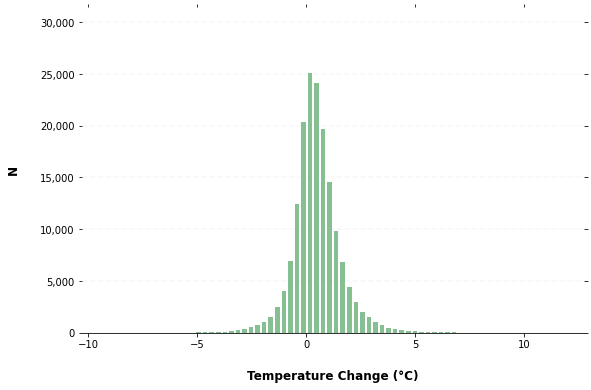
\includegraphics[scale=0.65]{fig/fig_1.png}
    \caption{Distribución de valores para el cambio de temperatura en $^o$C.}
    \vspace{-0.3cm}
    \source{Elaboración propia}
    \label{fig:fig_1}
\end{figure}\\
Se observa que los valores distribuyen normalmente con un coeficiente de curtosis positivo, y si bien a priori se podría creer que el promedio es en un valor cercano al 0, en realidad es en un valor más cércano a $0,5$.\\ \\
El promedio y varianza de la totalida de los datos es:
\begin{multicols}{2}
\begin{itemize}
    \item \textbf{Promedio:} $0.478\ ^o$C
    \item \textbf{Varianza:} $1.218\ (^o$C)$^2$
\end{itemize}
\end{multicols}
El valor positivo en la media se interpreta como un aumento mes a mes del cambio en la temperatura.\\ \\
Para observar la evolución de los cambios de temperatura a medida avanza el flujo de tiempo, observemos una serie de tiempo en donde se desagrega por continente el cambio de temperatura promedio, agregandole además una serie para la evolución del cambio de temperatura en el mundo:
\begin{figure}[H]
    \centering
    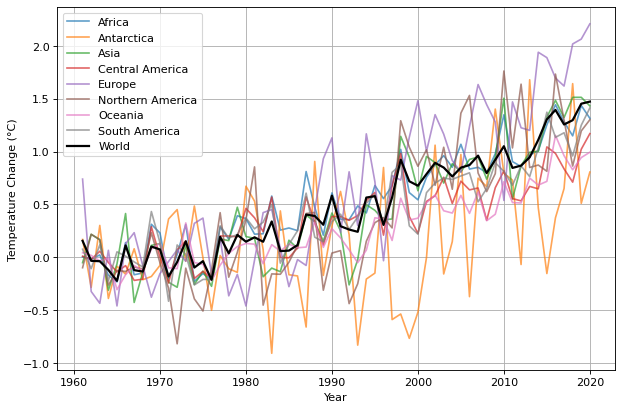
\includegraphics[scale=0.5]{fig/fig_2.png}
    \caption{Series temporales para el cambio de temperatura.}
    \vspace{-0.3cm}
    \source{Elaboración propia}
    \label{fig:fig_1}
\end{figure}\\
Podemos observar que la Antartica ofusca un poco los datos, por lo que separaremos este fenómeno en dos gráficos para ver otra comparación:
\begin{figure}[H]
     \centering
     \begin{subfigure}[b]{0.45\textwidth}
         \centering
         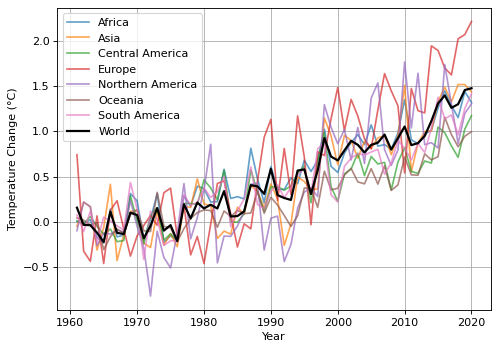
\includegraphics[width=\textwidth]{fig/fig_3.png}
         \caption{Series Temporales Continentes.}
    \label{fig:fig_1}
     \end{subfigure}
     \hfill
     \begin{subfigure}[b]{0.45\textwidth}
         \centering
         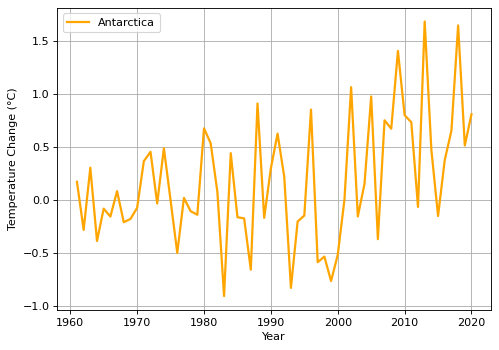
\includegraphics[width=\textwidth]{fig/fig_4.png}
         \caption{Serie temporal Antártica.}
    \label{fig:fig_1}
     \end{subfigure}
        \caption{Series temporales para el cambio de temperatura. Desagregado.}
        \vspace{-0.3cm}
        \source{Elaboración propia}
    \label{fig:fig_1}
\end{figure}\\
En todos los casos se observa un crecimiento paulatino de el cambio de temperatura a medida avanza el tiempo, incluso en el caso de la Antártica, donde el comportamiento es irregular.\\
Si bien lo anterior nos da indicios de como esta aumentando el cambio de temperatura año a año, veamos como se comportan las distribuciones mensuales históricas y como se comportan en los últimos 10 años mediante gráficos del tipo boxplot:
\begin{figure}[H]
     \centering
     \begin{subfigure}[b]{0.45\textwidth}
         \centering
         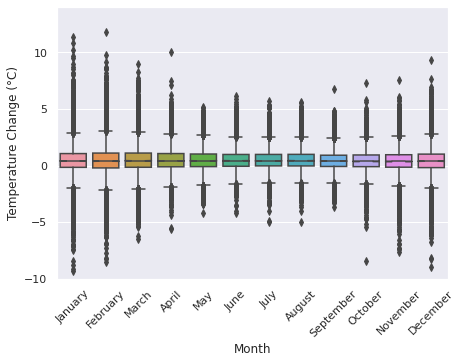
\includegraphics[width=\textwidth]{fig/fig_5.png}
         \caption{Datos históricos.}
    \label{fig:fig_1}
     \end{subfigure}
     \hfill
     \begin{subfigure}[b]{0.45\textwidth}
         \centering
         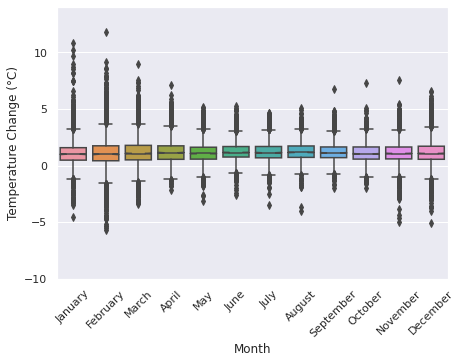
\includegraphics[width=\textwidth]{fig/fig_6.png}
         \caption{Datos de los últimos 10 años.}
    \label{fig:fig_1}
     \end{subfigure}
        \caption{Distribución mensual de los cambios de temperatura.}
        \vspace{-0.3cm}
        \source{Elaboración propia}
    \label{fig:fig_1}
\end{figure}\\
\vspace{-0.6cm}
De los gráficos se desprende que las medias mensuales son mayores en los últimos 10 años que en los datos históricos, además los máximos se repiten y los mínimos desaparecen en el último tramo. Lo anterior  para el caso histórico se puede visualizar con más detalle en la siguiente tabla:
\begin{table}[H]
    \centering
    \begin{tcolorbox}[tab2,tabularx={s||s|s|s|s},title=Estadísticas mensuales,boxrule=0.5pt]
        \textsc{Mes} & \textsc{Min.}     & \textsc{Max.}     & \textsc{Prom.}     & \textsc{Var.}      \\\hline\hline
        Enero               & -9.303 $^o$C	&11.332 $^o$C	&0.473 $^o$C	&1.845 $(^o$C)$^2$  \\\hline
        Febrero	            & -8.485 $^o$C	&11.759 $^o$C	&0.490 $^o$C	&2.199 $(^o$C)$^2$  \\\hline
        Marzo               & -6.491 $^o$C	&9.012 $^o$C	&0.530 $^o$C	&1.621 $(^o$C)$^2$  \\\hline
        Abril               & -5.622 $^o$C	&10.049 $^o$C	&0.513 $^o$C	&1.092 $(^o$C)$^2$  \\\hline
        Mayo	            & -4.201 $^o$C	&5.213 $^o$C	&0.488 $^o$C	&0.932 $(^o$C)$^2$  \\\hline
        Junio	            & -4.203 $^o$C	&6.167 $^o$C	&0.494 $^o$C	&0.804 $(^o$C)$^2$  \\\hline
        Julio	            & -5.023 $^o$C	&5.709 $^o$C	&0.521 $^o$C	&0.810 $(^o$C)$^2$  \\\hline
        Agosto              & -4.991 $^o$C	&5.576 $^o$C	&0.532 $^o$C	&0.828 $(^o$C)$^2$   \\\hline
        Septiembre	        & -3.668 $^o$C  &6.735 $^o$C	&0.447 $^o$C	&0.788 $(^o$C)$^2$ \\\hline
        Octubre	            & -8.405 $^o$C	&7.248 $^o$C	&0.439 $^o$C	&0.942 $(^o$C)$^2$  \\\hline
        Noviembre	        & -7.670 $^o$C	&7.580 $^o$C	&0.401 $^o$C	&1.218 $(^o$C)$^2$ \\\hline
        Diciembre           & -8.960 $^o$C	&9.306 $^o$C	&0.403 $^o$C	&1.519 $(^o$C)$^2$  
    \end{tcolorbox}
    \caption{Estadísticas históricas para cada mes.}
    \label{tab:table_1}
\end{table}\\
Para realizar un análisis un poco mas desagregado, analizemos país a país los estadísticos descriptivos principales. A continuación se muestran gráficos de tipo boxplot para los 10 países con mayores temperaturas y para los 10 países con menores temperaturas registradas. 
\begin{figure}[H]
    \centering
    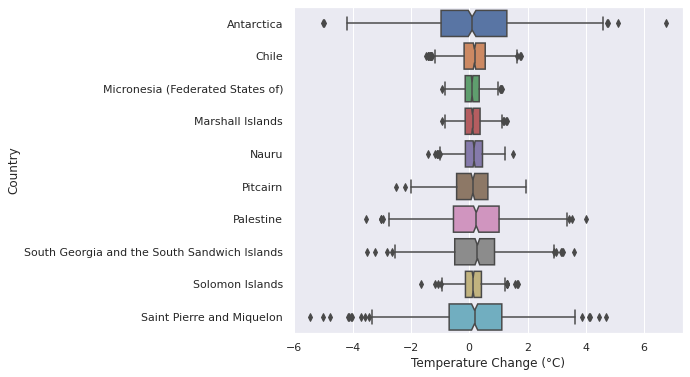
\includegraphics[scale=0.5]{fig/fig_7.png}
    \caption{Países con los menores cambios de temperatura.}
    \vspace{-0.3cm}
    \source{Elaboración propia}
    \label{fig:fig_1}
\end{figure}\\
\begin{figure}[H]
    \centering
    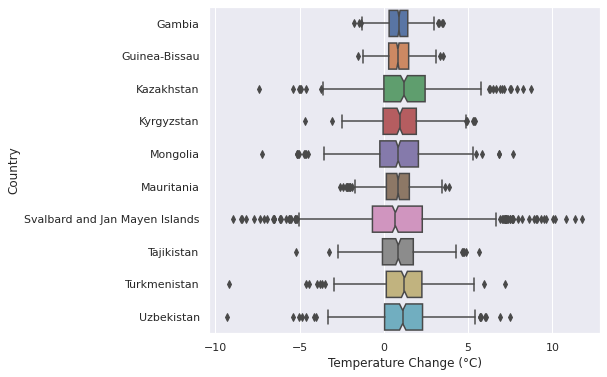
\includegraphics[scale=0.5]{fig/fig_8.png}
    \caption{Países con los mayores cambios de temperatura.}
    \vspace{-0.3cm}
    \source{Elaboración propia}
    \label{fig:fig_1}
\end{figure}\\
Si bien acá solo registramos los países con menores y mayores cambios, en el apéndice se encuentra una tabla más detallada con todos los países.

\section{Conclusiones}  
En consecuencia del análisis de datos realizado, entre las principales conclusiones obtenidas fueron:
\begin{itemize}
    \item Los graficos en su conjunto develan la existencia de una evidente alza en el cambio de temperatura. Esto es evidente desde las series temporales hasta los promedios desagregados.
    \item En la antartica, el cambio abrupto desprendido del gráfico que muestra la variación de temperatura por región da cuenta de manera contraintuitiva que es la región más afectada por el cambio climático.
    \item  Entre los paises que menor alza de temperatura tienen podemos encontrar a Chile, micronesia, etc. Esto puede ser debido a que son islas o países que se encuentran cerca del océano, lo que actua como un regulador natural de temperatura.
    \item Los países que mas alza presentan se hayan en asia, esto puede ser debido a la deslocalización que realizan las empresas a fin de abaratar costos en la producción, la que mayormente se realiza en países de escasos recursos.
    \item El hecho de que exista un alza en países de escasos recursos invita a reflexionar acerca de como el cambio climático incrementa la probreza, dado que las personas se ven forzadas a emigrar, las tierras de cultivo se estropean, las oportunidades laborales disminuyen y no existe acceso a servicios básicos como el agua potable y la sanidad.
\end{itemize}



%-----------os márginales para los 100 datos que venían en el ------------n como los efect-----------------------------------------------------------------
%	REFERENCES
%------------------------------

\newpage
\phantomsection
\pagenumbering{roman}
\addcontentsline{toc}{section}{R \ Referencias}
\bibliographystyle{apacite}
\bibliography{myrefs.bib}

\addcontentsline{toc}{section}{A \ Apéndice}
\section*{Apéndice}
\begin{table}[H]
    \centering
    \begin{tcolorbox}[tab2,tabularx={s||s|s|s|s},title=Estadísticas para África I,boxrule=0.5pt]
        \textsc{País} & \textsc{Min.}     & \textsc{Max.}     & \textsc{Prom.}     & \textsc{Var.}       \\\hline\hline
        Algeria   &   -2.769  $^o$  &   4.297  $^o$  &   0.714  $^o$  &   1.455 $(^o$C)$^2$ \\\hline
Angola   &   -1.208  $^o$  &   2.958  $^o$  &   0.466  $^o$  &   0.438 $(^o$C)$^2$ \\\hline
Benin   &   -1.942  $^o$  &   2.205  $^o$  &   0.515  $^o$  &   0.443 $(^o$C)$^2$ \\\hline
Botswana   &   -2.736  $^o$  &   3.406  $^o$  &   0.385  $^o$  &   1.054 $(^o$C)$^2$ \\\hline
Burkina Faso   &   -2.427  $^o$  &   3.088  $^o$  &   0.564  $^o$  &   0.699 $(^o$C)$^2$ \\\hline
Burundi   &   -2.51  $^o$  &   3.236  $^o$  &   0.528  $^o$  &   0.453 $(^o$C)$^2$ \\\hline
Cote d'Ivoire   &   -1.165  $^o$  &   2.387  $^o$  &   0.585  $^o$  &   0.376 $(^o$C)$^2$ \\\hline
Cabo Verde   &   -3.621  $^o$  &   3.429  $^o$  &   0.66  $^o$  &   0.72 $(^o$C)$^2$ \\\hline
Cameroon   &   -1.84  $^o$  &   2.637  $^o$  &   0.47  $^o$  &   0.415 $(^o$C)$^2$ \\\hline
Central African Republic   &   -2.428  $^o$  &   4.074  $^o$  &   0.494  $^o$  &   0.545 $(^o$C)$^2$ \\\hline
Chad   &   -3.466  $^o$  &   4.464  $^o$  &   0.481  $^o$  &   0.918 $(^o$C)$^2$ \\\hline
Comoros   &   -1.096  $^o$  &   1.959  $^o$  &   0.241  $^o$  &   0.268 $(^o$C)$^2$ \\\hline
Congo   &   -1.118  $^o$  &   1.853  $^o$  &   0.386  $^o$  &   0.317 $(^o$C)$^2$ \\\hline
Democratic Republic of the Congo   &   -0.835  $^o$  &   2.089  $^o$  &   0.448  $^o$  &   0.33 $(^o$C)$^2$ \\\hline
Djibouti   &   -2.714  $^o$  &   4.092  $^o$  &   0.579  $^o$  &   0.709 $(^o$C)$^2$ \\\hline
Egypt   &   -3.224  $^o$  &   3.903  $^o$  &   0.348  $^o$  &   1.336 $(^o$C)$^2$ \\\hline
Equatorial Guinea   &   -1.368  $^o$  &   2.159  $^o$  &   0.391  $^o$  &   0.299 $(^o$C)$^2$ \\\hline
Eritrea   &   -3.085  $^o$  &   4.108  $^o$  &   0.491  $^o$  &   0.6 $(^o$C)$^2$ \\\hline
Eswatini   &   -2.913  $^o$  &   2.721  $^o$  &   0.298  $^o$  &   0.665 $(^o$C)$^2$ \\\hline
Ethiopia   &   -0.660796  $^o$  &   3.057  $^o$  &   0.55  $^o$  &   0.341 $(^o$C)$^2$ \\\hline
French Southern Territories   &   -2.53  $^o$  &   2.538  $^o$  &   0.335  $^o$  &   0.53 $(^o$C)$^2$ \\\hline
Gabon   &   -0.923  $^o$  &   2.405  $^o$  &   0.356  $^o$  &   0.338 $(^o$C)$^2$ \\\hline
Gambia   &   -1.772  $^o$  &   3.517  $^o$  &   0.864  $^o$  &   0.681 $(^o$C)$^2$ \\\hline
Ghana   &   -1.37  $^o$  &   2.195  $^o$  &   0.554  $^o$  &   0.35 $(^o$C)$^2$ \\\hline
Guinea   &   -1.039  $^o$  &   2.963  $^o$  &   0.677  $^o$  &   0.508 $(^o$C)$^2$ \\\hline
Guinea-Bissau   &   -1.516  $^o$  &   3.535  $^o$  &   0.874  $^o$  &   0.681 $(^o$C)$^2$\\\hline
Kenya   &   -1.317  $^o$  &   2.974  $^o$  &   0.424  $^o$  &   0.364 $(^o$C)$^2$ 
    \end{tcolorbox}
    \caption{Estadísticas históricas para el continente Africano I.}
    \label{tab:table_1}
\end{table}\\



\begin{table}[H]
    \centering
    \begin{tcolorbox}[tab2,tabularx={s||s|s|s|s},title=Estadísticas para África II,boxrule=0.5pt]
        \textsc{País} & \textsc{Min.}     & \textsc{Max.}     & \textsc{Prom.}     & \textsc{Var.}       \\\hline\hline
Lesotho   &   -2.23  $^o$  &   4.236  $^o$  &   0.43  $^o$  &   0.743 $(^o$C)$^2$ \\\hline
Liberia   &   -0.991  $^o$  &   2.391  $^o$  &   0.616  $^o$  &   0.39 $(^o$C)$^2$ \\\hline
Libya   &   -3.048  $^o$  &   3.793  $^o$  &   0.392  $^o$  &   1.46 $(^o$C)$^2$ \\\hline
Madagascar   &   -1.134  $^o$  &   2.588  $^o$  &   0.406  $^o$  &   0.359 $(^o$C)$^2$ \\\hline
Malawi   &   -1.471  $^o$  &   3.439  $^o$  &   0.441  $^o$  &   0.526 $(^o$C)$^2$ \\\hline
Mali   &   -2.117  $^o$  &   3.958  $^o$  &   0.637  $^o$  &   0.853 $(^o$C)$^2$ \\\hline
Mauritania   &   -2.569  $^o$  &   3.871  $^o$  &   0.823  $^o$  &   1.122 $(^o$C)$^2$ \\\hline
Mauritius   &   -1.098  $^o$  &   2.307  $^o$  &   0.522  $^o$  &   0.372 $(^o$C)$^2$ \\\hline
Mayotte   &   -1.687  $^o$  &   2.137  $^o$  &   0.303  $^o$  &   0.325 $(^o$C)$^2$ \\\hline
Morocco   &   -3.008  $^o$  &   4.483  $^o$  &   0.743  $^o$  &   1.705 $(^o$C)$^2$ \\\hline
Mozambique   &   -1.88  $^o$  &   2.3  $^o$  &   0.331  $^o$  &   0.42 $(^o$C)$^2$ \\\hline
Namibia   &   -2.057  $^o$  &   3.565  $^o$  &   0.346  $^o$  &   0.74 $(^o$C)$^2$ \\\hline
Niger   &   -3.584  $^o$  &   4.384  $^o$  &   0.575  $^o$  &   1.274 $(^o$C)$^2$ \\\hline
Nigeria   &   -2.839  $^o$  &   3.36  $^o$  &   0.537  $^o$  &   0.658 $(^o$C)$^2$ \\\hline
R?union   &   -1.343  $^o$  &   2.586  $^o$  &   0.495  $^o$  &   0.426 $(^o$C)$^2$ \\\hline
Rwanda   &   -2.51  $^o$  &   2.364  $^o$  &   0.528  $^o$  &   0.413 $(^o$C)$^2$ \\\hline
Saint Helena   &   -1.695  $^o$  &   3.012  $^o$  &   0.717  $^o$  &   0.643 $(^o$C)$^2$ \\\hline
Sao Tome and Principe   &   -1.175  $^o$  &   2.412  $^o$  &   0.402  $^o$  &   0.293 $(^o$C)$^2$ \\\hline
Senegal   &   -2.011  $^o$  &   3.531  $^o$  &   0.799  $^o$  &   0.673 $(^o$C)$^2$ \\\hline
Seychelles   &   -1.211  $^o$  &   2.217  $^o$  &   0.479  $^o$  &   0.369 $(^o$C)$^2$ \\\hline
Sierra Leone   &   -1.069  $^o$  &   2.932  $^o$  &   0.739  $^o$  &   0.62 $(^o$C)$^2$ \\\hline
Somalia   &   -1.478  $^o$  &   3.695  $^o$  &   0.624  $^o$  &   0.575 $(^o$C)$^2$ \\\hline
South Africa   &   -2.234  $^o$  &   3.157  $^o$  &   0.481  $^o$  &   0.616 $(^o$C)$^2$ \\\hline
South Sudan   &   -1.049  $^o$  &   2.891  $^o$  &   0.519  $^o$  &   0.343 $(^o$C)$^2$ \\\hline
Sudan   &   -1.508667  $^o$  &   3.827  $^o$  &   0.584  $^o$  &   0.816 $(^o$C)$^2$ \\\hline
Togo   &   -1.273  $^o$  &   2.198  $^o$  &   0.521  $^o$  &   0.372 $(^o$C)$^2$ \\\hline
Tunisia   &   -2.634  $^o$  &   4.671  $^o$  &   0.734  $^o$  &   1.61 $(^o$C)$^2$ \\\hline
Uganda   &   -1.514  $^o$  &   2.846  $^o$  &   0.431  $^o$  &   0.385 $(^o$C)$^2$ \\\hline
United Republic of Tanzania   &   -1.238  $^o$  &   2.239  $^o$  &   0.408  $^o$  &   0.35 $(^o$C)$^2$ \\\hline
Western Sahara   &   -3.1  $^o$  &   4.522  $^o$  &   0.796  $^o$  &   1.44 $(^o$C)$^2$ \\\hline
Zambia   &   -1.657  $^o$  &   3.565  $^o$  &   0.453  $^o$  &   0.61 $(^o$C)$^2$ \\\hline
Zimbabwe   &   -2.33  $^o$  &   3.004  $^o$  &   0.315  $^o$  &   0.738 $(^o$C)$^2$ 

    \end{tcolorbox}
    \caption{Estadísticas históricas para el continente Africano II.}
    \label{tab:table_1}
\end{table}\\



\begin{table}[H]
    \centering
    \begin{tcolorbox}[tab2,tabularx={s||s|s|s|s},title=Estadísticas para Asia I,boxrule=0.5pt]
        \textsc{País} & \textsc{Min.}     & \textsc{Max.}     & \textsc{Prom.}     & \textsc{Var.}       \\\hline\hline
Afghanistan   &   -7.724  $^o$  &   4.803  $^o$  &   0.477  $^o$  &   2 $(^o$C)$^2$ \\\hline
Armenia   &   -4.619  $^o$  &   5.612  $^o$  &   0.499  $^o$  &   2.029 $(^o$C)$^2$ \\\hline
Azerbaijan   &   -5.448  $^o$  &   5.873  $^o$  &   0.492  $^o$  &   1.882 $(^o$C)$^2$ \\\hline
Bahrain   &   -3.62  $^o$  &   4.298  $^o$  &   0.685  $^o$  &   1.663 $(^o$C)$^2$ \\\hline
Bangladesh   &   -2.244  $^o$  &   4.015  $^o$  &   0.28  $^o$  &   0.575 $(^o$C)$^2$ \\\hline
Bhutan   &   -2.063  $^o$  &   3.321  $^o$  &   0.335  $^o$  &   0.689 $(^o$C)$^2$ \\\hline
Brunei Darussalam   &   -1.41  $^o$  &   2.193  $^o$  &   0.363  $^o$  &   0.273 $(^o$C)$^2$ \\\hline
Cambodia   &   -2.069  $^o$  &   2.521  $^o$  &   0.41  $^o$  &   0.456 $(^o$C)$^2$ \\\hline
China   &   -2.789  $^o$  &   4.381  $^o$  &   0.557  $^o$  &   0.898 $(^o$C)$^2$ \\\hline
China, Hong Kong SAR   &   -4.9  $^o$  &   6.114  $^o$  &   0.401  $^o$  &   1.455 $(^o$C)$^2$ \\\hline
China, Macao SAR   &   -4.9  $^o$  &   6.114  $^o$  &   0.401  $^o$  &   1.455 $(^o$C)$^2$ \\\hline
Cyprus   &   -3.835  $^o$  &   4.266  $^o$  &   0.424  $^o$  &   1.442 $(^o$C)$^2$ \\\hline
Democratic People's Republic of Korea   &   -4.38  $^o$  &   5.717  $^o$  &   0.635  $^o$  &   1.923 $(^o$C)$^2$ \\\hline
Georgia   &   -5.653  $^o$  &   5.307  $^o$  &   0.427  $^o$  &   2.033 $(^o$C)$^2$ \\\hline
India   &   -1.743  $^o$  &   2.555  $^o$  &   0.275  $^o$  &   0.393 $(^o$C)$^2$ \\\hline
Indonesia   &   -0.628  $^o$  &   1.767  $^o$  &   0.327  $^o$  &   0.181 $(^o$C)$^2$ \\\hline
Iran (Islamic Republic of)   &   -6  $^o$  &   4.574  $^o$  &   0.636  $^o$  &   1.67 $(^o$C)$^2$ \\\hline
Iraq   &   -5.151  $^o$  &   5.529  $^o$  &   0.501  $^o$  &   1.953 $(^o$C)$^2$ \\\hline
Israel   &   -3.532  $^o$  &   4.025  $^o$  &   0.24  $^o$  &   1.424 $(^o$C)$^2$ \\\hline
Japan   &   -2.758  $^o$  &   2.916  $^o$  &   0.328  $^o$  &   0.882 $(^o$C)$^2$ \\\hline
Jordan   &   -3.435  $^o$  &   4.812  $^o$  &   0.243  $^o$  &   1.736 $(^o$C)$^2$ \\\hline
Kazakhstan   &   -7.385  $^o$  &   8.707  $^o$  &   1.26  $^o$  &   5.224 $(^o$C)$^2$ \\\hline
Kuwait   &   -5.118  $^o$  &   4.664  $^o$  &   0.689  $^o$  &   2.046 $(^o$C)$^2$ \\\hline
Kyrgyzstan   &   -4.68  $^o$  &   5.433  $^o$  &   1.014  $^o$  &   2.395 $(^o$C)$^2$
    \end{tcolorbox}
    \caption{Estadísticas históricas para el continente Asiatico I.}
    \label{tab:table_1}
\end{table}\\



\begin{table}[H]
    \centering
    \begin{tcolorbox}[tab2,tabularx={s||s|s|s|s},title=Estadísticas para Asia II,boxrule=0.5pt]
        \textsc{País} & \textsc{Min.}     & \textsc{Max.}     & \textsc{Prom.}     & \textsc{Var.}       \\\hline\hline
Kyrgyzstan   &   -4.68  $^o$  &   5.433  $^o$  &   1.014  $^o$  &   2.395 $(^o$C)$^2$ \\\hline
Lao People's Democratic Republic   &   -2.622  $^o$  &   3.305  $^o$  &   0.439  $^o$  &   0.773 $(^o$C)$^2$ \\\hline
Lebanon   &   -3.798  $^o$  &   4.717  $^o$  &   0.368  $^o$  &   1.57 $(^o$C)$^2$ \\\hline
Malaysia   &   -0.894  $^o$  &   2.2  $^o$  &   0.432  $^o$  &   0.251 $(^o$C)$^2$ \\\hline
Maldives   &   -2.973  $^o$  &   1.613  $^o$  &   0.341  $^o$  &   0.251 $(^o$C)$^2$ \\\hline
Mongolia   &   -7.248  $^o$  &   7.652  $^o$  &   0.875  $^o$  &   3.391 $(^o$C)$^2$ \\\hline
Myanmar   &   -1.617  $^o$  &   2.753  $^o$  &   0.469  $^o$  &   0.492 $(^o$C)$^2$ \\\hline
Nepal   &   -2.214  $^o$  &   4.162  $^o$  &   0.255  $^o$  &   0.706 $(^o$C)$^2$ \\\hline
Oman   &   -4.278  $^o$  &   3.211  $^o$  &   0.411  $^o$  &   0.732 $(^o$C)$^2$ \\\hline
Pakistan   &   -4.483  $^o$  &   4.347  $^o$  &   0.272  $^o$  &   1.061 $(^o$C)$^2$ \\\hline
Palestine   &   -3.546  $^o$  &   4.023  $^o$  &   0.237  $^o$  &   1.431 $(^o$C)$^2$ \\\hline
Philippines   &   -1.117  $^o$  &   1.966  $^o$  &   0.46  $^o$  &   0.266 $(^o$C)$^2$ \\\hline
Qatar   &   -3.61  $^o$  &   3.814  $^o$  &   0.637  $^o$  &   1.434 $(^o$C)$^2$ \\\hline
Republic of Korea   &   -4.104  $^o$  &   4.256  $^o$  &   0.454  $^o$  &   1.473 $(^o$C)$^2$ \\\hline
Saudi Arabia   &   -3.343  $^o$  &   3.962  $^o$  &   0.445  $^o$  &   1.283 $(^o$C)$^2$ \\\hline
Singapore   &   -1.236  $^o$  &   2.776  $^o$  &   0.522  $^o$  &   0.415 $(^o$C)$^2$ \\\hline
Sri Lanka   &   -0.988  $^o$  &   2.06  $^o$  &   0.484  $^o$  &   0.274 $(^o$C)$^2$ \\\hline
Syrian Arab Republic   &   -4.164  $^o$  &   4.791  $^o$  &   0.424  $^o$  &   1.946 $(^o$C)$^2$ \\\hline
Tajikistan   &   -5.214  $^o$  &   5.648  $^o$  &   0.881  $^o$  &   2.132 $(^o$C)$^2$ \\\hline
Thailand   &   -2.416  $^o$  &   2.834  $^o$  &   0.444  $^o$  &   0.566 $(^o$C)$^2$ \\\hline
Timor-Leste   &   -2.348  $^o$  &   2.952  $^o$  &   0.344  $^o$  &   0.473 $(^o$C)$^2$ \\\hline
Turkey   &   -4.379  $^o$  &   4.799  $^o$  &   0.421  $^o$  &   2.316 $(^o$C)$^2$ \\\hline
Turkmenistan   &   -9.157  $^o$  &   7.178  $^o$  &   1.135  $^o$  &   3.297 $(^o$C)$^2$ \\\hline
United Arab Emirates   &   -3.383  $^o$  &   3.651  $^o$  &   0.459  $^o$  &   1.194 $(^o$C)$^2$ \\\hline
Uzbekistan   &   -9.303  $^o$  &   7.491  $^o$  &   1.091  $^o$  &   4.181 $(^o$C)$^2$ \\\hline
Viet Nam   &   -2.378  $^o$  &   3.241  $^o$  &   0.39  $^o$  &   0.661 $(^o$C)$^2$ \\\hline
Yemen   &   -2.726118  $^o$  &   3.901412  $^o$  &   0.541  $^o$  &   0.863 $(^o$C)$^2$ 
    \end{tcolorbox}
    \caption{Estadísticas históricas para el continente Asiatico II.}
    \label{tab:table_1}
\end{table}\\



\begin{table}[H]
    \centering
    \begin{tcolorbox}[tab2,tabularx={s||s|s|s|s},title=Estadísticas para Europa I,boxrule=0.5pt]
        \textsc{País} & \textsc{Min.}     & \textsc{Max.}     & \textsc{Prom.}     & \textsc{Var.}       \\\hline\hline
Albania   &   -4.334  $^o$  &   4.807  $^o$  &   0.488  $^o$  &   2.104 $(^o$C)$^2$ \\\hline
Andorra   &   -4.555  $^o$  &   5.576  $^o$  &   0.69  $^o$  &   2.262 $(^o$C)$^2$ \\\hline
Austria   &   -5.3  $^o$  &   5.639  $^o$  &   0.787  $^o$  &   3.206 $(^o$C)$^2$ \\\hline
Belarus   &   -6.881  $^o$  &   8.136  $^o$  &   0.748  $^o$  &   4.651 $(^o$C)$^2$ \\\hline
Belgium   &   -5.168  $^o$  &   5.865  $^o$  &   0.711  $^o$  &   2.586 $(^o$C)$^2$ \\\hline
Bosnia and Herzegovina   &   -4.409  $^o$  &   5.147  $^o$  &   0.643  $^o$  &   2.001 $(^o$C)$^2$ \\\hline
Bulgaria   &   -5.709  $^o$  &   6.305  $^o$  &   0.499  $^o$  &   2.843 $(^o$C)$^2$ \\\hline
Croatia   &   -3.935  $^o$  &   4.997  $^o$  &   0.685  $^o$  &   1.984 $(^o$C)$^2$ \\\hline
Czechia   &   -5.87975  $^o$  &   6.206  $^o$  &   0.688  $^o$  &   3.359 $(^o$C)$^2$ \\\hline
Denmark   &   -6.076  $^o$  &   6.571  $^o$  &   0.688  $^o$  &   3.332 $(^o$C)$^2$ \\\hline
Estonia   &   -5.595  $^o$  &   8.72  $^o$  &   0.74  $^o$  &   3.877 $(^o$C)$^2$ \\\hline
Faroe Islands   &   -3.486  $^o$  &   3.425  $^o$  &   0.376  $^o$  &   1.183 $(^o$C)$^2$ \\\hline
Finland   &   -8.742  $^o$  &   9.74  $^o$  &   0.772  $^o$  &   6.238 $(^o$C)$^2$ \\\hline
France   &   -4.601  $^o$  &   5.193  $^o$  &   0.683  $^o$  &   2.213 $(^o$C)$^2$ \\\hline
Germany   &   -6.676  $^o$  &   5.841  $^o$  &   0.731  $^o$  &   3.33 $(^o$C)$^2$ \\\hline
Gibraltar   &   -2.536  $^o$  &   4.159  $^o$  &   0.627  $^o$  &   1.353 $(^o$C)$^2$ \\\hline
Greece   &   -3.796  $^o$  &   4.226  $^o$  &   0.334  $^o$  &   1.538 $(^o$C)$^2$ \\\hline
Holy See   &   -3.612  $^o$  &   5.006  $^o$  &   0.575  $^o$  &   1.719 $(^o$C)$^2$ \\\hline
Hungary   &   -5.487  $^o$  &   6.473  $^o$  &   0.641  $^o$  &   3.514 $(^o$C)$^2$ \\\hline
Iceland   &   -4.282  $^o$  &   4.278  $^o$  &   0.343  $^o$  &   1.73 $(^o$C)$^2$ \\\hline
Ireland   &   -4.427  $^o$  &   3.443  $^o$  &   0.397  $^o$  &   1.304 $(^o$C)$^2$ \\\hline
Isle of Man   &   -4.748  $^o$  &   3.878  $^o$  &   0.399  $^o$  &   1.457 $(^o$C)$^2$ \\\hline
Italy   &   -3.419  $^o$  &   4.924  $^o$  &   0.62  $^o$  &   1.636 $(^o$C)$^2$ \\\hline
Latvia   &   -5.648  $^o$  &   8.494  $^o$  &   0.721  $^o$  &   3.775 $(^o$C)$^2$ \\\hline
Liechtenstein   &   -4.887  $^o$  &   5.851  $^o$  &   0.77  $^o$  &   3.055 $(^o$C)$^2$ \\\hline
Lithuania   &   -5.801  $^o$  &   8.158  $^o$  &   0.71  $^o$  &   3.775 $(^o$C)$^2$ \\\hline
Luxembourg   &   -5.168  $^o$  &   5.945  $^o$  &   0.733  $^o$  &   2.789 $(^o$C)$^2$ \\\hline
Malta   &   -2.777  $^o$  &   3.551  $^o$  &   0.563  $^o$  &   1.176 $(^o$C)$^2$ \\\hline
Monaco   &   -4.081  $^o$  &   4.997  $^o$  &   0.651  $^o$  &   1.693 $(^o$C)$^2$ \\\hline
Montenegro   &   -4.735  $^o$  &   5.32  $^o$  &   0.627  $^o$  &   1.623 $(^o$C)$^2$ \\\hline
Netherlands   &   -7.124  $^o$  &   6.179  $^o$  &   0.703  $^o$  &   3.103 $(^o$C)$^2$ 
    \end{tcolorbox}
    \caption{Estadísticas históricas para el continente Europeo I.}
    \label{tab:table_1}
\end{table}\\



\begin{table}[H]
    \centering
    \begin{tcolorbox}[tab2,tabularx={s||s|s|s|s},title=Estadísticas para Europa II,boxrule=0.5pt]
        \textsc{País} & \textsc{Min.}     & \textsc{Max.}     & \textsc{Prom.}     & \textsc{Var.}       \\\hline\hline
North Macedonia   &   -5.509  $^o$  &   5.59  $^o$  &   0.527  $^o$  &   1.737 $(^o$C)$^2$ \\\hline
Norway   &   -5.826  $^o$  &   7.301  $^o$  &   0.636  $^o$  &   3.476 $(^o$C)$^2$ \\\hline
Poland   &   -7.422  $^o$  &   7.243  $^o$  &   0.695  $^o$  &   4.264 $(^o$C)$^2$ \\\hline
Portugal   &   -3.309  $^o$  &   4.575  $^o$  &   0.634  $^o$  &   1.734 $(^o$C)$^2$ \\\hline
Republic of Moldova   &   -6.577  $^o$  &   7.093  $^o$  &   0.602  $^o$  &   3.734 $(^o$C)$^2$ \\\hline
Romania   &   -6.915  $^o$  &   6.682  $^o$  &   0.545  $^o$  &   3.402 $(^o$C)$^2$ \\\hline
Russian Federation   &   -5.87975  $^o$  &   7.392  $^o$  &   0.749  $^o$  &   3.251 $(^o$C)$^2$ \\\hline
San Marino   &   -3.823  $^o$  &   5.586  $^o$  &   0.676  $^o$  &   2.178 $(^o$C)$^2$ \\\hline
Serbia   &   -5.299  $^o$  &   6.009  $^o$  &   0.637  $^o$  &   1.686 $(^o$C)$^2$ \\\hline
Slovakia   &   -5.87975  $^o$  &   6.57  $^o$  &   0.619  $^o$  &   3.275 $(^o$C)$^2$ \\\hline
Slovenia   &   -3.393  $^o$  &   5.549  $^o$  &   0.772  $^o$  &   2.208 $(^o$C)$^2$ \\\hline
Spain   &   -3.003  $^o$  &   4.16  $^o$  &   0.684  $^o$  &   1.464 $(^o$C)$^2$ \\\hline
Svalbard and Jan Mayen Islands   &   -8.96  $^o$  &   11.759  $^o$  &   0.872  $^o$  &   9.32 $(^o$C)$^2$ \\\hline
Sweden   &   -7  $^o$  &   8.544  $^o$  &   0.73  $^o$  &   4.57 $(^o$C)$^2$ \\\hline
Switzerland   &   -5.024  $^o$  &   6.167  $^o$  &   0.744  $^o$  &   2.869 $(^o$C)$^2$ \\\hline
Ukraine   &   -7.387  $^o$  &   7.305  $^o$  &   0.632  $^o$  &   3.859 $(^o$C)$^2$ \\\hline
United Kingdom of Great Britain and Northern I...   &   -4.432  $^o$  &   3.776  $^o$  &   0.432  $^o$  &   1.443 $(^o$C)$^2$
    \end{tcolorbox}
    \caption{Estadísticas históricas para el continente Europeo II.}
    \label{tab:table_1}
\end{table}\\



\begin{table}[H]
    \centering
    \begin{tcolorbox}[tab2,tabularx={s||s|s|s|s},title=Estadísticas para Antártica,boxrule=0.5pt]
        \textsc{País} & \textsc{Min.}     & \textsc{Max.}     & \textsc{Prom.}     & \textsc{Var.}       \\\hline\hline
Antarctica   &   -5.023  $^o$  &   6.735  $^o$  &   0.176  $^o$  &   2.961 $(^o$C)$^2$ 
    \end{tcolorbox}
    \caption{Estadísticas históricas para el continente Antártico.}
    \label{tab:table_1}
\end{table}\\



\begin{table}[H]
    \centering
    \begin{tcolorbox}[tab2,tabularx={s||s|s|s|s},title=Estadísticas para Norteamérica,boxrule=0.5pt]
        \textsc{País} & \textsc{Min.}     & \textsc{Max.}     & \textsc{Prom.}     & \textsc{Var.}       \\\hline\hline
Canada   &   -6.324  $^o$  &   6.138  $^o$  &   0.619  $^o$  &   2.626 $(^o$C)$^2$ \\\hline
Greenland   &   -6.338  $^o$  &   6.826  $^o$  &   0.388  $^o$  &   3.139 $(^o$C)$^2$ \\\hline
Mexico   &   -1.58  $^o$  &   2.632  $^o$  &   0.372  $^o$  &   0.474 $(^o$C)$^2$ \\\hline
Saint Pierre and Miquelon   &   -5.446  $^o$  &   4.699  $^o$  &   0.188  $^o$  &   2.03 $(^o$C)$^2$ \\\hline
United States of America   &   -3.513  $^o$  &   3.828  $^o$  &   0.47  $^o$  &   0.964 $(^o$C)$^2$     \end{tcolorbox}
    \caption{Estadísticas históricas para América del Norte.}
    \label{tab:table_1}
\end{table}\\



\begin{table}[H]
    \centering
    \begin{tcolorbox}[tab2,tabularx={s||s|s|s|s},title=Estadísticas para Sudamérica,boxrule=0.5pt]
        \textsc{País} & \textsc{Min.}     & \textsc{Max.}     & \textsc{Prom.}     & \textsc{Var.}       \\\hline\hline
Argentina   &   -2.595  $^o$  &   3.18  $^o$  &   0.266  $^o$  &   0.787 $(^o$C)$^2$ \\\hline
Bolivia (Plurinational State of)   &   -1.969  $^o$  &   3.835  $^o$  &   0.603  $^o$  &   0.681 $(^o$C)$^2$ \\\hline
Brazil   &   -1.441  $^o$  &   2.298  $^o$  &   0.534  $^o$  &   0.368 $(^o$C)$^2$ \\\hline
Chile   &   -1.474  $^o$  &   1.774  $^o$  &   0.18  $^o$  &   0.302 $(^o$C)$^2$ \\\hline
Colombia   &   -1.265  $^o$  &   1.944  $^o$  &   0.297  $^o$  &   0.273 $(^o$C)$^2$ \\\hline
Ecuador   &   -1.341  $^o$  &   2.318  $^o$  &   0.393  $^o$  &   0.371 $(^o$C)$^2$ \\\hline
French Guyana   &   -0.655  $^o$  &   2.455  $^o$  &   0.602  $^o$  &   0.497 $(^o$C)$^2$ \\\hline
Guyana   &   -2.324  $^o$  &   2.433  $^o$  &   0.515  $^o$  &   0.462 $(^o$C)$^2$ \\\hline
Paraguay   &   -4.93  $^o$  &   3.996  $^o$  &   0.376  $^o$  &   1.523 $(^o$C)$^2$ \\\hline
Peru   &   -1.155  $^o$  &   2.208  $^o$  &   0.476  $^o$  &   0.325 $(^o$C)$^2$ \\\hline
Suriname   &   -0.981  $^o$  &   2.594  $^o$  &   0.64  $^o$  &   0.596 $(^o$C)$^2$ \\\hline
Uruguay   &   -3.021  $^o$  &   4.963  $^o$  &   0.391  $^o$  &   1.404 $(^o$C)$^2$ \\\hline
Venezuela (Bolivarian Republic of)   &   -1.149  $^o$  &   1.963  $^o$  &   0.312  $^o$  &   0.257 $(^o$C)$^2$ 
     \end{tcolorbox}
    \caption{Estadísticas históricas para América del Sur.}
    \label{tab:table_1}
\end{table}\\


\begin{table}[H]
    \centering
    \begin{tcolorbox}[tab2,tabularx={s||s|s|s|s},title=Estadísticas para Oceanía,boxrule=0.5pt]
        \textsc{País} & \textsc{Min.}     & \textsc{Max.}     & \textsc{Prom.}     & \textsc{Var.}       \\\hline\hline
American Samoa   &   -1.183  $^o$  &   2.395  $^o$  &   0.421  $^o$  &   0.343 $(^o$C)$^2$ \\\hline
Australia   &   -1.507  $^o$  &   3.127  $^o$  &   0.456  $^o$  &   0.609 $(^o$C)$^2$ \\\hline
Christmas Island   &   -0.996  $^o$  &   2.054  $^o$  &   0.306  $^o$  &   0.301 $(^o$C)$^2$ \\\hline
Cocos (Keeling) Islands   &   -1.133  $^o$  &   2.368  $^o$  &   0.299  $^o$  &   0.34 $(^o$C)$^2$ \\\hline
Cook Islands   &   -1.466  $^o$  &   2.619  $^o$  &   0.32  $^o$  &   0.326 $(^o$C)$^2$ \\\hline
Fiji   &   -1.661  $^o$  &   2.024  $^o$  &   0.287  $^o$  &   0.363 $(^o$C)$^2$ \\\hline
French Polynesia   &   -1.035  $^o$  &   1.466  $^o$  &   0.242  $^o$  &   0.158 $(^o$C)$^2$ \\\hline
Kiribati   &   -0.831  $^o$  &   2.722  $^o$  &   0.272  $^o$  &   0.262 $(^o$C)$^2$ \\\hline
Marshall Islands   &   -0.9465  $^o$  &   1.283  $^o$  &   0.124  $^o$  &   0.139 $(^o$C)$^2$ \\\hline
Micronesia (Federated States of)   &   -0.9465  $^o$  &   1.122  $^o$  &   0.107  $^o$  &   0.125 $(^o$C)$^2$ \\\hline
Nauru   &   -1.417  $^o$  &   1.504  $^o$  &   0.15  $^o$  &   0.211 $(^o$C)$^2$ \\\hline
New Caledonia   &   -1.266  $^o$  &   3.102  $^o$  &   0.348  $^o$  &   0.489 $(^o$C)$^2$ \\\hline
New Zealand   &   -2.321  $^o$  &   3.571  $^o$  &   0.27  $^o$  &   0.682 $(^o$C)$^2$ \\\hline
Niue   &   -1.337  $^o$  &   1.827  $^o$  &   0.291  $^o$  &   0.319 $(^o$C)$^2$ \\\hline
Norfolk Island   &   -1.324  $^o$  &   2.279  $^o$  &   0.339  $^o$  &   0.404 $(^o$C)$^2$ \\\hline
Palau   &   -0.9465  $^o$  &   1.753  $^o$  &   0.262  $^o$  &   0.235 $(^o$C)$^2$ \\\hline
Papua New Guinea   &   -1.244  $^o$  &   1.853  $^o$  &   0.315  $^o$  &   0.218 $(^o$C)$^2$ \\\hline
Pitcairn   &   -2.513  $^o$  &   1.96  $^o$  &   0.08  $^o$  &   0.55 $(^o$C)$^2$ \\\hline
Samoa   &   -1.157  $^o$  &   2.311  $^o$  &   0.332  $^o$  &   0.314 $(^o$C)$^2$ \\\hline
Solomon Islands   &   -1.65  $^o$  &   1.681  $^o$  &   0.149  $^o$  &   0.182 $(^o$C)$^2$ \\\hline
Tokelau   &   -1.049  $^o$  &   1.756667  $^o$  &   0.324  $^o$  &   0.239 $(^o$C)$^2$ \\\hline
Tonga   &   -1.338  $^o$  &   2.249  $^o$  &   0.312  $^o$  &   0.384 $(^o$C)$^2$ \\\hline
Tuvalu   &   -1.094  $^o$  &   1.6  $^o$  &   0.253  $^o$  &   0.219 $(^o$C)$^2$ \\\hline
Vanuatu   &   -1.236  $^o$  &   2.413  $^o$  &   0.273  $^o$  &   0.31 $(^o$C)$^2$ \\\hline
Wallis and Futuna Islands   &   -1.253  $^o$  &   1.972  $^o$  &   0.286  $^o$  &   0.298 $(^o$C)$^2$
     \end{tcolorbox}
    \caption{Estadísticas históricas para Oceanía.}
    \label{tab:table_1}
\end{table}\\



\begin{table}[H]
    \centering
    \begin{tcolorbox}[tab2,tabularx={s||s|s|s|s},title=Estadísticas para Centromérica I,boxrule=0.5pt]
        \textsc{País} & \textsc{Min.}     & \textsc{Max.}     & \textsc{Prom.}     & \textsc{Var.}       \\\hline\hline
Anguilla   &   -1.204  $^o$  &   2.184  $^o$  &   0.298  $^o$  &   0.227 $(^o$C)$^2$ \\\hline
Antigua and Barbuda   &   -1.231  $^o$  &   2.387  $^o$  &   0.292  $^o$  &   0.231 $(^o$C)$^2$ \\\hline
Aruba   &   -1.385  $^o$  &   2.07  $^o$  &   0.366  $^o$  &   0.295 $(^o$C)$^2$ \\\hline
Bahamas   &   -3.333  $^o$  &   3.774  $^o$  &   0.484  $^o$  &   0.679 $(^o$C)$^2$ \\\hline
Barbados   &   -1.315  $^o$  &   2.272  $^o$  &   0.303  $^o$  &   0.278 $(^o$C)$^2$ \\\hline
Belize   &   -2.022  $^o$  &   3.92  $^o$  &   0.448  $^o$  &   0.891 $(^o$C)$^2$ \\\hline
British Virgin Islands   &   -1.335  $^o$  &   1.98  $^o$  &   0.304  $^o$  &   0.253 $(^o$C)$^2$ \\\hline
Cayman Islands   &   -2.691  $^o$  &   2.957  $^o$  &   0.448  $^o$  &   0.434 $(^o$C)$^2$ \\\hline
Costa Rica   &   -1.595  $^o$  &   2.401  $^o$  &   0.315  $^o$  &   0.384 $(^o$C)$^2$ \\\hline
Cuba   &   -2.223  $^o$  &   2.895  $^o$  &   0.51  $^o$  &   0.488 $(^o$C)$^2$ \\\hline
Dominica   &   -1.197  $^o$  &   2.282  $^o$  &   0.288  $^o$  &   0.219 $(^o$C)$^2$ \\\hline
Dominican Republic   &   -1.316  $^o$  &   2.196  $^o$  &   0.464  $^o$  &   0.32 $(^o$C)$^2$ \\\hline
El Salvador   &   -1.245  $^o$  &   2.837  $^o$  &   0.439  $^o$  &   0.371 $(^o$C)$^2$ \\\hline
Falkland Islands (Malvinas)   &   -2.517  $^o$  &   1.981  $^o$  &   0.364  $^o$  &   0.352 $(^o$C)$^2$ \\\hline
Grenada   &   -1.105  $^o$  &   1.952  $^o$  &   0.294  $^o$  &   0.226 $(^o$C)$^2$ \\\hline
Guadeloupe   &   -1.138  $^o$  &   2.246  $^o$  &   0.293  $^o$  &   0.213 $(^o$C)$^2$ \\\hline
Guatemala   &   -1.854  $^o$  &   2.968  $^o$  &   0.446  $^o$  &   0.405 $(^o$C)$^2$ \\\hline
Haiti   &   -1.661  $^o$  &   2.187  $^o$  &   0.55  $^o$  &   0.402 $(^o$C)$^2$ \\\hline
Honduras   &   -1.471  $^o$  &   3.595  $^o$  &   0.472  $^o$  &   0.439 $(^o$C)$^2$ \\\hline
Jamaica   &   -1.257  $^o$  &   2.164  $^o$  &   0.56  $^o$  &   0.368 $(^o$C)$^2$ \\\hline
Martinique   &   -1.206  $^o$  &   2.207  $^o$  &   0.291  $^o$  &   0.217 $(^o$C)$^2$ \\\hline
Montserrat   &   -1.231  $^o$  &   2.387  $^o$  &   0.292  $^o$  &   0.231 $(^o$C)$^2$ \\\hline
Nicaragua   &   -1.89  $^o$  &   2.534  $^o$  &   0.415  $^o$  &   0.364 $(^o$C)$^2$ \\\hline
Panama   &   -0.871  $^o$  &   1.872  $^o$  &   0.303  $^o$  &   0.283 $(^o$C)$^2$ \\\hline
Puerto Rico   &   -1.395  $^o$  &   1.851  $^o$  &   0.366  $^o$  &   0.265 $(^o$C)$^2$ \\\hline
Saint Kitts and Nevis   &   -1.231  $^o$  &   2.387  $^o$  &   0.292  $^o$  &   0.231 $(^o$C)$^2$ 
     \end{tcolorbox}
    \caption{Estadísticas históricas para América Central I.}
    \label{tab:table_1}
\end{table}\\



\begin{table}[H]
    \centering
    \begin{tcolorbox}[tab2,tabularx={s||s|s|s|s},title=Estadísticas para Centromérica II,boxrule=0.5pt]
        \textsc{País} & \textsc{Min.}     & \textsc{Max.}     & \textsc{Prom.}     & \textsc{Var.}       \\\hline\hline
Saint Lucia   &   -1.073  $^o$  &   2.033  $^o$  &   0.294  $^o$  &   0.205 $(^o$C)$^2$ \\\hline
Saint Vincent and the Grenadines   &   -1.115  $^o$  &   1.94  $^o$  &   0.293  $^o$  &   0.226 $(^o$C)$^2$ \\\hline
South Georgia and the South Sandwich Islands   &   -3.498  $^o$  &   3.61  $^o$  &   0.223  $^o$  &   1.147 $(^o$C)$^2$ \\\hline
Trinidad and Tobago   &   -1.249  $^o$  &   2.251  $^o$  &   0.315  $^o$  &   0.27 $(^o$C)$^2$ \\\hline
Turks and Caicos Islands   &   -1.508  $^o$  &   1.7829  $^o$  &   0.397  $^o$  &   0.238 $(^o$C)$^2$ \\\hline
United States Virgin Islands   &   -1.348  $^o$  &   1.962  $^o$  &   0.314  $^o$  &   0.252 $(^o$C)$^2$ 
     \end{tcolorbox}
    \caption{Estadísticas históricas para América Central II.}
    \label{tab:table_1}
\end{table}\\





\end{document}